\documentclass[tikz,border=8pt]{standalone}
\usepackage{braket}

\begin{document}
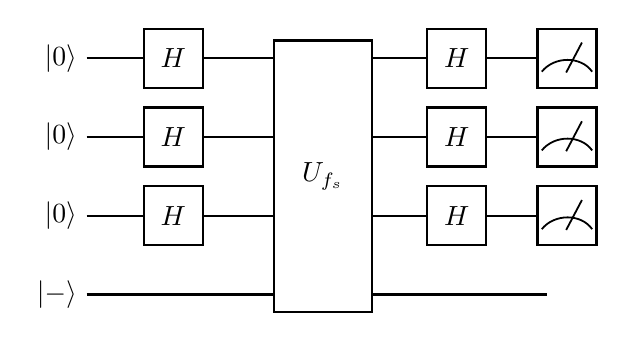
\begin{tikzpicture}[
  wire/.style={line width=0.8pt},
  gate/.style={draw,fill=white,line width=0.8pt,
    minimum width=0.75cm,minimum height=0.75cm,inner sep=0pt},
  oracle/.style={draw,fill=white,line width=0.8pt,
    minimum width=1.25cm,minimum height=3.45cm,inner sep=0pt}
]
  % Three input qubits and one auxiliary qubit.
  \foreach \y in {1.35,0.35,-0.65} {
    \draw[wire] (0,\y) -- (6.1,\y);
    \node[left] at (0,\y) {$\ket{0}$};
    \node[gate] at (1.1,\y) {$H$};
    \node[gate] at (4.7,\y) {$H$};
    \node[gate] at (6.1,\y) {};
    % Computational-basis measurement symbol.
    \draw[line width=0.65pt] (5.78,\y-0.17)
      .. controls (5.94,\y+0.03) and (6.28,\y+0.03) .. (6.42,\y-0.17);
    \draw[line width=0.65pt] (6.09,\y-0.18) -- (6.29,\y+0.20);
  }
  \draw[wire] (0,-1.65) -- (5.85,-1.65);
  \node[left] at (0,-1.65) {$\ket{-}$};

  % U_f acts on the input register and the auxiliary qubit.
  \node[oracle] at (3.0,-0.15) {$U_{f_s}$};
\end{tikzpicture}
\end{document}
